\section{Ricostruzione degli episodi}
\label{sec:secondo-punto}
\subsection{Cronologia essenziale e componenti coinvolti}
L'8 settembre 2025 l'account npm del manutentore di pacchetti Josh, è stato compromesso a seguito di un attacco di phishing, portando alla pubblicazione di versioni malevole di pacchetti.
Alle 13:16 UTC, i sistemi di Aikido Security hanno rilevato la pubblicazione di diversi pacchetti npm contenenti codice sospetto, l'azienda ha successivamente avvisato il manutentore.

Poche ore dopo lo stesso utente ha dichiarato di aver perso il controllo dell'account e di essere al lavoro per risolvere il problema. Secondo Aikido il manutentore sembrava essere riuscito a rimuovere parte dei pacchetti compromessi prima di perdere l'accesso al proprio account.
Nello stesso giorno inoltre, furono aperte anche alcune issue sui repository GitHub, come la issue 656 per chalk 5.6.1 e la 1005 per debug 4.4.2, per segnalare la presenza di codice malevolo nelle versioni appena pubblicate su npm e per avvertire gli sviluppatori.
\cite{aikido2025}
\cite{chalk2025}
\begin{figure}[H]
    \centering
    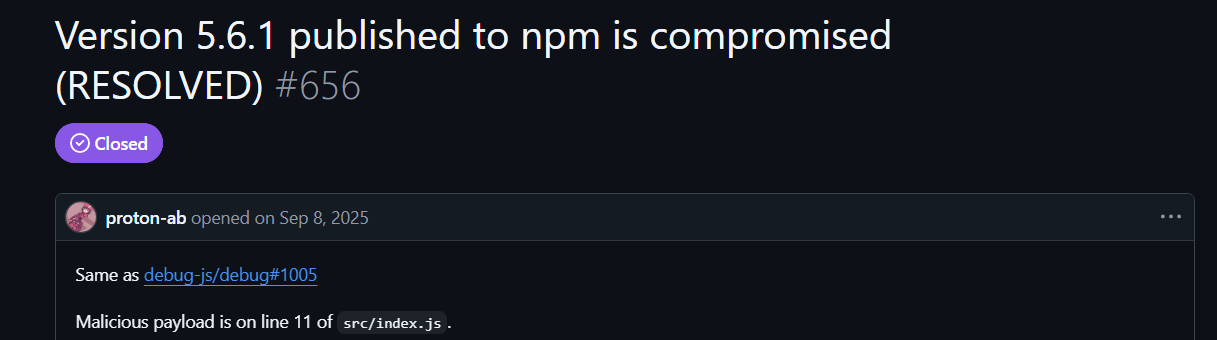
\includegraphics[width=0.75\textwidth]{immagine_compromesso_chalk.png}
    \caption{Issue GitHub relativa alla compromissione del pacchetto chalk@5.6.1.}
    {\footnotesize Fonte: \cite{chalk2025}\par}
    \label{fig:issue-chalk}
\end{figure}
\subsection{Risposta adottata}
Durante la giornata dell'8 Settembre npm ha rimosso le versioni compromesse dei pacchetti per evitare ulteriori download.
La patch correttiva per debug arriva solamente il 13 Settembre, quando il manutentore rilascia la versione sicura 4.4.3 accompagnata da alcune indicazioni per gli sviluppatori: aggiornare i pacchetti alle versioni sicure, eliminare completamente la cartella \texttt{node\_modules}, svuotare la cache del gestore dei pacchetti e ricostruire da zero i bundle creati con i pacchetti compromessi.
\cite{debug2025}
% Sviluppare il secondo aspetto del tema e il collegamento con il primo.
% Inserire analisi, confronti o un caso di studio, secondo il tema scelto.
